% Intended LaTeX compiler: pdflatex
\documentclass[10pt,a4paper,UTF8]{article}
\usepackage{zclorg}
\author{张朝龙}
\date{}
\title{练习:零空间和值域}
\hypersetup{
 pdfauthor={张朝龙},
 pdftitle={练习:零空间和值域},
 pdfkeywords={},
 pdfsubject={},
 pdfcreator={Emacs 25.0.50.1 (Org mode 9.0.5)}, 
 pdflang={English}}
\begin{document}

\maketitle
\tableofcontents
\titlepic{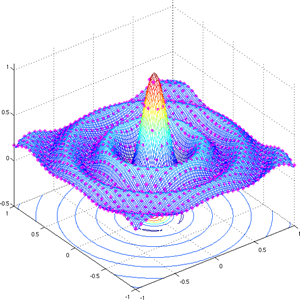
\includegraphics[scale=0.25]{../../img/sinc.PNG}}


\section{3.B.1}
\label{sec:org9766077}


\begin{problem}
给出线性映射\(T\)使得\(\dim nullT = 3\)且\(\dim range T = 2\)
\end{problem}

\begin{answer}


根据线性映射基本定理\(\dim V = \dim nullT + \dim rangeT\),有\(\dim V = 5\). 

所以我们可以定义一个维度为5的向量空间\(V= \mathbf{R}^{5}\),并令这个空间的基为\(e_{1},\ldots ,e_{5}\),其中\(e_{i}\)是第\(i\)个元素为\(1\),其他元素为零的向量。接下来我们定义线性映射\(T\):
\begin{eqnarray}
\label{eq:1}
T(e_{1}) &=& 0 \\
T(e_{2}) &=&0 \\
T(e_{3}) &=&0 \\
T(e_{4}) &=& e_{5}\\
T(e_{5}) &=& e_{4}
\end{eqnarray}

根据线性映射的定义,我们可以证明\(T\)是线性映射,满足齐次可加性。另外根据定义,\(e_{1},e_{2},e_{3}\in nullT\),并且\(nullT = span(e_{1},e_{2},e_{3})\),所以\(\dim nullT = 3\),根据线性映射基本定理\(\dim rangeT = 2\)


注意我们定义线性映射\(T\)的时候最好写成定义线性映射\(T: \mathcal{L}(V,V)\),即\(T\)是自身到自身的映射。
\end{answer}
\section{3.B.2}
\label{sec:orgca976d2}


\begin{problem}
设\(V\)是向量空间,\(S,T\in \mathcal{L}(V,V)\)使得\(range S\subset nullT\),证明\((ST)^{2} = 0\)
\end{problem}

\begin{answer}
因为\(range S \subset nullT\),所以对于任何\(s\in rangeS\)有\(Ts = 0\),所以有\(TS = 0\),对于\((ST)^{2}\),我们可以展开如下:
\begin{eqnarray*}
(ST)^{2}&=&(ST)(ST) \\
&=&S(TS)T \\
&=&S0T \\
&=&0
\end{eqnarray*}
\end{answer}

\section{3.B.3}
\label{sec:org3598b5e}


\begin{problem}
设\(v_{1},\ldots ,v_{m}\)是\(V\)中的向量组,定义\(T\in \mathcal{L}( \mathbf{F}^{m},V)\),如下:\[T(z_{1},\ldots ,z_{m}) = z_{1}v_{1} + \ldots + z_{m}v_{m}\]

\begin{enumerate}
\item \(T\)的什么性质相当于\(v_{1},\ldots ,v_{m}\)张成\(V\)?
\item \(T\)的什么性质相当于\(v_{1},\ldots ,v_{m}\)是线性无关的?
\end{enumerate}
\end{problem}

\begin{answer}
\begin{enumerate}
\item 相当于\(T\)满足什么条件才有\(span(v_{1},\ldots ,v_{m}) = V\)?我们知道张成组的定义是指\(V\)中的任意向量都可以写成\(v_{1},\ldots ,v_{m}\)的线性组合。而对于:\[T(z_{1},\ldots ,z_{m}) = z_{1}v_{1} + \ldots + z_{m}v_{m}\] 说明\(T\)的值域是\(v_{1},\ldots ,v_{m}\)的线性组合。即\(range T = \{v:v = z_{1}v_{1} + \ldots + z_{m}v_{m}\}\),只要\(range T = V\)和\(span(v_{1},\ldots ,v_{m}) = V\)是等效的。即\(T\)是满射。

\item \(v_{1},\ldots ,v_{m}\)是线性无关的相当于\(z_{1}v_{1} +  \ldots + z_{m}v_{m}=0\)只有一种写法\(z_{i}=0\)。这意味着\((z_{1},\ldots ,z_{m}) = \underbrace{(0,\ldots ,0)}_{m}\),即对于\(T\)来说只有\(T0 = 0\)。显然\(T\)必须有\(nullT = \{0\}\),即\(T\)是单射。
\end{enumerate}
\end{answer}

\section{3.B.4}
\label{sec:org508de5d}


\begin{problem}
证明\(\{T\in \mathcal{L}(\mathbf{R}^{5}, \mathbf{R}^{4}):\dim nullT >2\}\)不是\(\mathcal{L}(\mathbf{R}^{5}, \mathbf{R}^{4})\)的子空间。
\end{problem}

\begin{answer}
因为\(\dim nullT = \dim \mathbf{R}^{5} - \dim rangeT\),且\(\dim range T = \dim \mathbf{R}^{4} = 4\),所以有\(\dim nullT = 1\). 所以\(\mathcal{L}(\mathbf{R}^{5}, \mathbf{R}^{4})\)是\(nullT =1,rangeT=4\)构成的线性映射组成的空间。\(\{T\in \mathcal{L}(\mathbf{R}^{5}, \mathbf{R}^{4}):\dim nullT >2\}\)和\(\{T\in \mathcal{L}(\mathbf{R}^{5}, \mathbf{R}^{4}):\dim nullT =1\}\)是互斥的,证明完毕。

看了答案之后,发现答案中直接给出了一个特例。有时候举出一个反例会大大的简化证明。

后来仔细想想我的证明过程有一个地方出现了差错:我武断的认为\(\dim range T = \dim \mathbf{R}^{4} = 4\),其实题目并没有说\(T\)是满射。\(\dim range T\)不一定等于\(\dim \mathbf{R}^{4} = 4\). 所以还是给定一个反例比较好。
\end{answer}

\section{3.B.5}
\label{sec:orgb6e0e43}


\begin{problem}
给出线性映射\(T: \mathbf{R}^{4} \rightarrow \mathbf{R}^{4}\),使得\(range T = null T\)
\end{problem}

\begin{answer}
因为\(\dim \mathbf{R}^{4} = 4\),\(range T = null T\) 根据线性映射基本定理,\(\dim range T = \dim null T = 2\)所以这个映射是存在的。

假设\(e_{1},e_{2},e_{3},e_{4}\)是\(\mathbf{R}^{4}\)的一个基,定义\(T: \mathbf{R}^{4} \rightarrow \mathbf{R}^{4}\)满足:
\begin{eqnarray*}
T(e_{1})&=& 0\\
T(e_{2})&=& 0\\
T(e_{3})&=& e_{1}\\
T(e_{4})&=& e_{2}\\
\end{eqnarray*}

则有 \(nullT = range T = \{e_{1},e_{2}\}\)
\end{answer}
\section{3.B.6}
\label{sec:orgbd4d91b}


\begin{problem}
证明不存在线性映射\(T: \mathbf{R}^{5} \rightarrow \mathbf{R}^{5}\),使得\(range T = nullT\)
\end{problem}

\begin{answer}
假设存在这样的线性映射\(T\),满足\(range T = nullT\),即\(\dim range T = \dim null T\)。根据线性映射基本定理\(\dim \mathbf{R}^{5} =5\),有\(\dim range T = \dim range null T = 2.5\),这是不可能的。矛盾。得证。
\end{answer}

\section{3.B.7}
\label{sec:org4d7cf5c}


\begin{problem}
设\(V\)和\(W\)都是有限维的,且\(2\leq \dim V \leq \dim W\)。证明\(\{T\in \mathcal{L}(V,W): nullT \neq {0}\}\) 不是\(\mathcal{L}(V,W)\)的子空间。
\end{problem}

\begin{answer}
假设\(v_{1},\ldots ,v_{n}\)是\(V\)的一个基,\(w_{1},w_{m}\)是\(W\)的一个基,因为 \(2\leq \dim V \leq \dim W\) 所以\(2\leq n \leq m\)。

假设\(T_{1},T_{2}\in \{T\in \mathcal{L}(V,W): nullT \neq {0}\}\),并且对于\(T_{1}\)则有:
\begin{equation}
\label{eq:3}
T_{1}v_{1} = 0, T_{1}v_{i} = w_{i}, i = 2,\ldots ,n
\end{equation}

对于\(T_{2}\)有:
\begin{equation}
\label{eq:4}
T_{2}v_{1} = w_{1}, T_{2}v_{2} = 0, T_{2}v_{i}= w_{i}, i = 3,\ldots ,n
\end{equation}

但是我们有:
\begin{equation}
\label{eq:5}
(T_{1} + T_{2}) v_{1} = w_{1}, (T_{1} + T_{2}) v_{2} = v_{2}, (T_{1} + T_{2})v_{i} = 2w_{i}, i = 3,\ldots ,n
\end{equation}

因为\(w_{1},w_{2},2w_{i},i=3,\ldots ,n\)是线性无关的,则有\(T_{1}+T_{2}\)是单射,\(nullT = \{0\}\)。所以\(\{T\in \mathcal{L}(V,W): nullT \neq {0}\}\)不是\(\mathcal{L}(V,W)\)的子空间。
\end{answer}
\section{3.B.8}
\label{sec:orgcf3ce95}


\begin{problem}
设\(V\)和\(W\)都是有限维的,且\(\dim V \geq \dim W \geq 2\),证明\(\{T\in \mathcal{L}(V,W): range T \neq W\}\)不是\(\mathcal{L}(V,W)\)的子空间。
\end{problem}

\begin{answer}
假设\(v_{1},\ldots ,v_{n}\)是\(V\)的一个基,\(w_{1},w_{m}\)是\(W\)的一个基,因为 \(2\leq \dim W \leq \dim V\) 所以\(2\leq m \leq n\)。

假设\(T_{1},T_{2}\in \{T\in \mathcal{L}(V,W): range T \neq W\}\),并且对于\(T_{1}\)则有:

\begin{equation}
\label{eq:12}
T_{1}v_{1} = 0, T_{1}v_{i} = w_{i}, i = 2,\ldots ,m
\end{equation}
对于\(T_{2}\)有:
\begin{equation}
\label{eq:13}
T_{2}v_{1} = w_{1}, T_{2}v_{2} = 0, T_{2}v_{i}= w_{i}, i = 3,\ldots ,m
\end{equation}

但是我们有:
\begin{equation}
\label{eq:14}
(T_{1} + T_{2}) v_{1} = w_{1}, (T_{1} + T_{2}) v_{2} = v_{2}, (T_{1} + T_{2})v_{i} = 2w_{i}, i = 3,\ldots ,m
\end{equation}


因为\(w_{1},w_{2},2w_{i},i=3,\ldots ,m\)是线性无关的,则有\(T_{1}+T_{2}\)是满射,\(rangeT = W\)。所以\(\{T\in \mathcal{L}(V,W): range T \neq W\}\)不是\(\mathcal{L}(V,W)\)的子空间。
\end{answer}
\section{3.B.9}
\label{sec:org2029a39}


\begin{problem}
设\(T\in \mathcal{L}(V,W)\)是单的,\(v_{1},\ldots ,v_{n}\)在\(V\)中线性无关。证明\(Tv_{1},\ldots ,Tv_{n}\)在\(W\)中线性无关。
\end{problem}

\begin{answer}
按照线性组合的定义,假设存在\(a_{i}\)使得\[a_{1}Tv_{1} + \ldots + a_{n}Tv_{n} = 0\]

根据线性映射的齐次可加性有:
\[T(a_{1}v_{1} + \ldots + a_{n}v_{n}) = 0\]

显然\(a_{1}v_{1} + \ldots + a_{n}v_{n} \in nullT\)。又因为\(T\)是单的,则必有\(nullT = \{0\}\),所以:
\[a_{1}v_{1} + \ldots + a_{n}v_{n} = 0\]

又因为\(v_{1},\ldots ,v_{n}\)是线性无关的。根据线性无关的定义,必有\(a_{i}=0, \forall a_{i}\)

所以有\(Tv_{1},\ldots ,Tv_{n}\)是线性无关的。
\end{answer}

\section{3.B.10}
\label{sec:org5979b97}


\begin{problem}
设\(v_{1},\ldots ,v_{n}\)张成\(V\),并设\(T\in \mathcal{V,W}\),证明\(Tv_{1},\ldots ,Tv_{n}\)张成\(rangeT\)。
\end{problem}

\begin{answer}
因为\(v_{1},\ldots ,v_{n}\)张成\(V\),则有对于\(v\in V\)存在\(a_{i},\ldots ,a_{n}\)使得\[a_{1}v_{1} + \ldots + a_{1}v_{n} = v\] 

对两边进行线性映射,有:
\begin{eqnarray*}
T(a_{1}v_{1} + \ldots + a_{1}v_{n})&=& Tv\\
a_{1}Tv_{1} + \ldots + a_{1}Tv_{n} &==&Tv
\end{eqnarray*}
我们知道\(Tv \in rangeT\),又因为\(v\)的任意性,所以\(Tv_{1},\ldots ,Tv_{n}\)张成了\(range T\)
\end{answer}
\section{3.B.11}
\label{sec:org2f1e5c3}


\begin{problem}
设\(S_{1},\ldots ,S_{n}\)均为单的线性映射,且\(S_{1}S_{2}\ldots S_{n}\)有意义,证明\(S_{1}S_{2}\ldots S_{n}\)是单射。
\end{problem}

\begin{answer}
对于这个题目的证明我想采用数学归纳法。
显然当\(n=1\)的时候,原命题成立。

假设当\(n=m\)时,\(S_{1}S_{2}\ldots S_{m}\)是单射,令\(S=S_{1}S_{2}\ldots S_{m}\),则接下来证明\(SS_{m+1}\)是单射。

因为\(S_{m+1}\)是单射所以\(nullS_{m+1}=\{0\}\),假设\(SS_{m+1}\)不是单射,则必有\(v\neq 0, v\in nullSS_{m+1}\)使得 \(SS_{m+1} \neq 0\)。

\begin{eqnarray}
\label{eq:2}
SS_{m+1}v &=& 0 \\
S(S_{m+1}v) &=& 0
\end{eqnarray}
因为\(S\)是单射,所以\(S_{m+1}v = 0\),又因为\(S_{m+1}\)也是单射所以\(v=0\),矛盾。所以必有\(SS_{m+1}\)也是单射。


这个题目说明,单射的组合任然是单射。
\end{answer}
\section{3.B.12}
\label{sec:org6449440}


\begin{problem}
设\(T\)是有限维的,\(T\in \mathcal{L}(V,W)\).证明\(V\)有一个子空间\(U\)使得\(U\cap nullT = \{0\}\)且\(range T = \{Tu:u\in U\}\).
\end{problem}

\begin{answer}
这个题目采用了和2.43以及3.22相同的证明思路。刚开始,我想看答案。后来居然给想出来了。我发誓:以后一个题目不思考一个星期不看答案。必须改掉答案依赖症。更多的锻炼思考能力。闲话少说,接下来给出证明过程。

首先我们知道\(nullT\)是\(V\)的子空间,假设\(v_{1},\ldots ,v_{m}\)是\(nullT\)的一组基,则可以把这组基扩展为\(V\)的一组基:\(v_{1},\ldots ,v_{m},w_{1},\ldots ,w_{n}\),接下来我们考察\(U = span(w_{1},\ldots ,w_{n})\),首先我们知道\(w_{1},\ldots ,w_{n}\)是\(U\)的一组基(线性无关又张成\(U\))。

令\(u\in U\cap nullT\),则存在\(a_{1},\ldots ,a_{m}, b_{1},\ldots ,b_{n}\in \mathbf{F}\)使得:
\begin{equation}
\label{eq:6}
u = a_{1}v_{1} + \ldots + a_{m}v_{m} = b_{1}w_{1} + \ldots + b_{n}w_{n}
\end{equation}
得:
\begin{equation}
\label{eq:7}
a_{1}v_{1} + \ldots + a_{m}v_{m} - b_{1}w_{1} - \ldots - b_{n}w_{n} = 0
\end{equation}

因为\(v_{1},\ldots ,v_{m},w_{1},\ldots ,w_{n}\)线性相关,则有:
\[a_{i}=0,b_{j}=0,i=1,\ldots ,m,j= 1,\ldots ,n\]
所以\(u=0\),即\(U\cap nullT = \{0\}\).

我们知道\(range T = \{Tv:v\in V\}\),对任意的\(v\in V\)都存在\(a_{i}\in \mathbf{F},b_{j}\in \mathbf{F},i = 1,\ldots ,m;j=1,\ldots ,n\)使得:
\begin{equation}
\label{eq:8}
v = a_{1}v_{1} + \ldots + a_{m}v_{m} + b_{1}w_{1} + \ldots + b_{n}w_{n}
\end{equation}
得:
\begin{equation}
\label{eq:9}
Tv = T(b_{1}w_{1} + \ldots + b_{n}w_{n})
\end{equation}
上式右边没有了系数为\(a_{i}\)的项,是因为\(v_{i}\in nullT\). 又因为\(u=b_{1}w_{1}+ \ldots + b_{n}w_{n} \in U\),又因为\(v\)的任意性,所以:
\begin{equation}
\label{eq:10}
\{Tv:v\in V\} = \{Tu:u\in U\}
\end{equation}
即\(rangeT = \{Tu:u\in U\}\)

综上\(U = span(w_{1},\ldots ,w_{n})\)就是我们要找的V的子空间。
\end{answer}

\section{3.B.13}
\label{sec:org9725702}


\begin{problem}
设\(T\)是从\(\mathbf{F}^{4}\)到\(\mathbf{F}^{2}\)的线性映射使得\(nullT = \{(x_{1},x_{2},x_{3},x_{4})\in \mathbf{F}^{4}:x_{1} = 5x_{2},x_{3} = 7x_{4}\}\),证明\(T\)是满的。
\end{problem}

\begin{answer}
根据线性映射基本定理\(\dim V = \dim nullT + \dim rangeT\),结合\(\dim nullT = 2\)我们有\(\dim rangeT = 2\)。
\end{answer}
\section{3.B.14}
\label{sec:orgd4fe291}


\begin{problem}
设\(U\)是\(\mathbf{R}^{8}\)的一个\(3\)维子空间,\(T\)是\(\mathbf{R}^{8}\)到\(\mathbf{R}^{5}\)的一个线性映射使得\(nullT = U\),证明\(T\)是满的。
\end{problem}

\begin{answer}
根据线性映射基本定理,\(\dim V = \dim nullT + \dim rangeT\) ,我们有\(\dim rangeT = 8-3 = 5\).

线性映射基本定理用的非常广泛,要把其证明过程仔细掌握了。
\end{answer}

\section{3.B.15}
\label{sec:org67714ac}


\begin{problem}
证明不存在零空间等于\(\{(x_{1},x_{2},x_{3},x_{4},x_{5}) \in \mathbf{F}^{5}: x_{1} = 3x_{2},x_{3} = x_{4}=x_{5}\}\)的\(\mathbf{F}^{5}\)到\(\mathbf{F}^{2}\)的线性映射。
\end{problem}

\begin{answer}
这个证明还是重点使用线性映射基本定理。易知,题目中所给零空间的维度是\(2\),根据线性映射基本定理\(\dim V = \dim nullT + \dim rangeT\)。所以\(\dim rangeT = 3\). 而\(\mathbf{F}^{2}\)的维度是\(2\)。

在\(\mathbf{F}^{2}\)中不可能存在维度是\(3\)的空间。
\end{answer}
\section{3.B.16}
\label{sec:org2276525}


\begin{problem}
假设在\(V\)上存在一个线性映射,其零空间和值域都是有限维的,证明\(V\)是有限维的。
\end{problem}

\begin{answer}
线性映射基本定理:\(\dim V = \dim nullT + \dim rangeT\)
\end{answer}

\section{3.B.17}
\label{sec:org72fb00b}


\begin{problem}
设\(V\)和\(W\)都是有限维的。证明存在一个\(V\)到\(W\)的单的线性映射当且仅当\(\dim V \leq \dim W\)。
\end{problem}

\begin{answer}
单射的等价条件是\(nullT = \{0\}\),即\(\dim nullT = 0\)。根据线性映射基本定理:\[\dim nullT = \dim V -\dim range T\]
因为\(\dim range T \leq \dim W\),所以\(\dim nullT \geq \dim V - \dim W \leq 0\) 所以存在\(\dim nullT = 0\)的线性映射。
\end{answer}

\section{3.B.18}
\label{sec:org14b00a8}


\begin{problem}
设\(V\)和\(W\)都是有限维的。证明存在一个\(V\)到\(W\)的满的线性映射当且仅当\(\dim V \geq \dim W\)
\end{problem}

\begin{answer}
根据线性映射基本定理:
\begin{eqnarray*}
\dim W = \dim range T&=&\dim V - \dim nullT \\
&\leq &\dim V \\
\end{eqnarray*}

证明另外一个方向,当\(\dim V \geq \dim W\)时,存在\(V\)到\(W\)满射。设\(v_{1},\ldots ,v_{m}\)是\(V\)的一个基,\(w_{1},\ldots ,w_{n}\)是\(W\)的一个基。因为\(\dim V \geq \dim W\)则有\(m \geq n\)。定义线性映射使得:
\[T(a_{1}v_{1} + \ldots a_{m}v_{m}) = a_{1}w_{1} + \ldots a_{n}w_{n}\] 

因为\(m \geq n\),所以上式右边\(a_{n}w_{n}\)是有意义的。又因为\(w_{1},\ldots ,w_{n}\)是\(W\)的基。所以(range T = W)$\backslash$
\end{answer}

\section{3.B.19}
\label{sec:org1511951}


\begin{problem}
设\(V\)和\(W\)都是有限维的,且\(U\)是\(V\)的子空间。证明存在\(T\in \mathcal{L}(V,W)\)使得\(nullT = U\)当且仅当\(\dim U \geq \dim V -\dim W\)
\end{problem}

\begin{answer}
我们首先证明从\(T\in \mathcal{L}(V,W)\)和\(null T = U\)可以推出\(\dim U \geq \dim V -\dim W\).

根据线性映射基本定理,有:
\begin{eqnarray*}
\dim nullT&=&\dim V -\dim rangeT \\
&\geq& \dim V - \dim W \\
\end{eqnarray*}
结合\(\dim U  = \dim nullT\),所以有\[\dim U \geq \dim V - \dim W\]

然后我们从\(\dim U \geq \dim V - \dim W\)推出存在\(T\in \mathcal{L}(V,W)\)使得\(nullT = U\).

假设\(u_{1},\ldots ,u_{m}\)是\(U\)的一个基,把这个基扩展为\(V\)的一个基\(u_{1},\ldots ,u_{m},v_{1},\ldots ,v_{n}\),令\(w_{1},\ldots ,w_q\)是\(W\)的一个基。定义线性映射:
\begin{equation}
\label{eq:11}
T(a_{1}u_{1} + \ldots + a_{m}u_{m} + b_{1}v_{1} + \ldots b_{n}v_{n}) = b_{1}w_{1} + \ldots b_{n}w_{n}
\end{equation}
因为\(\dim U \geq \dim V - \dim W\)所以有\(q \geq n\),所以上式\(b_{n}w_{n}\)是有意义的。所以有\(nullT = U\)且\(T\in \mathcal{L}(V,W)\)
\end{answer}


\section{3.B.20}
\label{sec:orgc13c992}


\begin{problem}
设\(W\)是有限维的,\(T\in \mathcal{L}(V,W)\)。证明\(T\)是单的当且仅当存在\(S\in \mathcal{L}(V,W)\)使得\(ST\)是\(V\)上的恒等映射
\end{problem}
\end{document}
